\documentclass{article}
\usepackage{eecstex}
\usepackage{pgfplots}

\renewcommand{\thesection}{\Alph{section}}
\renewcommand{\thesubsection}{\thesection.\arabic{subsection}}

\title{EE 120 HW 01}
\author{Bryan Ngo}
\date{2021-01-22}

\begin{document}

\maketitle

\section{Euler's Formula}

\begin{equation}
    e^{i \theta} = \cos(\theta) + i \sin(\theta)
\end{equation}

\subsection{}

\begin{theorem}
    \begin{equation}
        \cos(\theta) = \frac{e^{i \theta} + e^{-i \theta}}{2}
    \end{equation}
\end{theorem}
\begin{proof}
    \begin{align}
        e^{-i \theta} &= \cos(-\theta) + i \sin(-\theta) \\
        &= \cos(\theta) - i \sin(\theta) \\
        &\Rightarrow e^{i \theta} + e^{-i \theta} = 2 \cos(\theta) \\
        &\Rightarrow \cos(\theta) = \frac{e^{i \theta} + e^{-i \theta}}{2}
    \end{align}
\end{proof}
\begin{theorem}
    \begin{equation}
        \sin(\theta) = \frac{e^{i \theta} - e^{-i \theta}}{2}
    \end{equation}
\end{theorem}
\begin{proof}
    \begin{align}
        e^{-i \theta} &= \cos(\theta) - i \sin(\theta) \\
        &\Rightarrow e^{i \theta} - e^{-i \theta} = 2 \sin(\theta) \\
        &\Rightarrow \sin(\theta) = \frac{e^{i \theta} - e^{-i \theta}}{2}
    \end{align}
\end{proof}

\subsection{}

\begin{theorem}
    \begin{equation}
        (\cos(\theta) + i \sin(\theta))^n = \cos(n \theta) + i \sin(n \theta)
    \end{equation}
\end{theorem}
\begin{proof}
    \begin{equation} 
        (\cos(\theta) + i \sin(\theta))^n = (e^{i \theta})^n = e^{i n \theta} = \cos(n \theta) + i \sin(n \theta)
    \end{equation}
\end{proof}

\subsection{}

\begin{theorem}
    \begin{equation}
        \sum_{k \in [1, N]} A_k \cos(\omega t + \phi_k) = A \cos(\omega t + \phi)
    \end{equation}
\end{theorem}
\begin{proof}
    \begin{align}
        \sum_{k \in [1, N]} A_k \cos(\omega t + \phi_k) &= \sum_{k \in [1, N]} A_k \frac{e^{i (\omega t + \phi_k)} + e^{-i (\omega t + \phi_k)}}{2} \\
        &= \sum_{k \in [1, N]} A_k e^{i \phi_k} \frac{e^{i \omega t} + e^{-i \omega t}}{2} \\
        &= \cos(\omega t) \sum_{k \in [1, N]} A_k e^{i \phi_k} \\
        &= \cos(\omega t) A e^{i \phi_k} = A \cos(\omega t + \phi_k)
    \end{align}
\end{proof}

\section{Periodicity of Signals}

\begin{enumerate}
    \item Yes, \(T = \frac{\pi}{2}\)
    \item Yes, \(T = 2\)
    \item No
    \item Yes, \(T = 4 \pi\)
    \item No
    \item No
    \item Yes, \(T = \frac{14}{6} = \frac{7}{3}\)
\end{enumerate}

\section{Signal Transformation}

\begin{center}
    \begin{tikzpicture}
        \begin{axis}[
            grid=both,
            xmin=-3, xmax=7,
            ymin=-1, ymax=3,
            xtick={0, 3, 5},
            ytick={0, 2},
            axis lines=middle,
            xlabel=\(x\), ylabel=\(y\),
            title=\(x(t)\)
        ]
        \addplot[
            color=blue,
            mark=none,
        ]
        coordinates {
            (-2, 0)
            (0, 0)
            (0, 2)
            (3, 0)
            (3, 2)
            (5, 0)
            (7, 0)
        };
        \end{axis}
    \end{tikzpicture}
\end{center}

\subsection{}

\begin{center}
    \begin{tikzpicture}
        \begin{axis}[
            grid=both,
            xmin=-7, xmax=3,
            ymin=-1, ymax=3,
            xtick={0, -3, -5},
            ytick={0, 2},
            axis lines=middle,
            xlabel=\(x\), ylabel=\(y\),
            title=\(x(-t)\)
        ]
        \addplot[
            color=blue,
            mark=none,
        ]
        coordinates {
            (2, 0)
            (0, 0)
            (0, 2)
            (-3, 0)
            (-3, 2)
            (-5, 0)
            (-7, 0)
        };
        \end{axis}
    \end{tikzpicture}
\end{center}

\subsection{}

\begin{center}
    \begin{tikzpicture}
        \begin{axis}[
            grid=both,
            xmin=-3, xmax=15,
            ymin=-1, ymax=3,
            xtick={0, 6, 10},
            ytick={0, 2},
            axis lines=middle,
            xlabel=\(x\), ylabel=\(y\),
            title=\(x(2t)\)
        ]
        \addplot[
            color=blue,
            mark=none,
        ]
        coordinates {
            (-2, 0)
            (0, 0)
            (0, 2)
            (6, 0)
            (6, 2)
            (10, 0)
            (14, 0)
        };
        \end{axis}
    \end{tikzpicture}
\end{center}

\subsection{}

\begin{center}
    \begin{tikzpicture}
        \begin{axis}[
            grid=both,
            xmin=-3, xmax=10,
            ymin=-1, ymax=3,
            xtick={2, 5, 7},
            ytick={0, 2},
            axis lines=middle,
            xlabel=\(x\), ylabel=\(y\),
            title=\(x(t + 2)\)
        ]
        \addplot[
            color=blue,
            mark=none,
        ]
        coordinates {
            (-2, 0)
            (2, 0)
            (2, 2)
            (5, 0)
            (5, 2)
            (7, 0)
            (9, 0)
        };
        \end{axis}
    \end{tikzpicture}
\end{center}

\subsection{}

\begin{center}
    \begin{tikzpicture}
        \begin{axis}[
            grid=both,
            xmin=-3, xmax=7,
            ymin=-1, ymax=3,
            xtick={-1, 0.5, 1.5},
            ytick={0, 2},
            axis lines=middle,
            xlabel=\(x\), ylabel=\(y\),
            title=\(x\left(\frac{t}{2} - 1\right)\)
        ]
        \addplot[
            color=blue,
            mark=none,
        ]
        coordinates {
            (-2, 0)
            (-1, 0)
            (-1, 2)
            (0.5, 0)
            (0.5, 2)
            (1.5, 0)
            (7, 0)
        };
        \end{axis}
    \end{tikzpicture}
\end{center}

\subsection{}

\begin{center}
    \begin{tikzpicture}
        \begin{axis}[
            grid=both,
            xmin=-15, xmax=5,
            ymin=-1, ymax=3,
            xtick={1, -8, -14},
            ytick={0, 2},
            axis lines=middle,
            xlabel=\(x\), ylabel=\(y\),
            title=\(x(1 - 3t)\)
        ]
        \addplot[
            color=blue,
            mark=none,
        ]
        coordinates {
            (5, 0)
            (1, 0)
            (1, 2)
            (-8, 0)
            (-8, 2)
            (-14, 0)
            (-15, 0)
        };
        \end{axis}
    \end{tikzpicture}
\end{center}

\section{Integral Review}

\subsection{}

\begin{equation}
    \int_{-1}^\infty e^{-2t} \, dt = \left.-\frac{1}{2} e^{-2t}\right|_{-1}^\infty = -\frac{1}{2} \lim_{R \to \infty} (\cancelto{0}{e^{-2R}} - e^2) = \frac{e^2}{2}
\end{equation}

\subsection{}

\begin{align}
    y(t) &= \int_{-\infty}^\infty u(\tau) e^{-a (t - \tau)} u(t - \tau) \, d\tau \\
    &= \int_0^\infty e^{-a (t - \tau)} u(t - \tau) \, d\tau
\end{align}
Letting \(v = t - \tau\), \(dv = -dt\).
Substituting into the integral,
\begin{align}
    \int_0^\infty e^{-a (t - \tau)} u(t - \tau) \, d\tau &= \int_t^{t - \infty} -e^{-a v} u(v) \, dv \\
    &=
    \begin{cases}
        \lim_{R \to \infty} \left.\frac{1}{a} e^{-a v}\right|_t^{t - R} & v > 0 \\
        0 & \text{elsewhere}
    \end{cases} \\
    &=
    \begin{cases}
        \frac{1}{a} \lim_{R \to \infty} \cancelto{0}{e^{a (t - R)}} - e^{-a t} & v > 0 \\
        0 & \text{elsewhere}
    \end{cases} \\
    &=
    \begin{cases}
        -\frac{1}{a} e^{-a t} & t > 0 \\
        0 & \text{elsewhere}
    \end{cases}
\end{align}

% TODO: fix this

\subsection{}

\begin{equation}
    X(\omega) = \int_{-\infty}^\infty e^{-a |t|} e^{-i \omega t} \, dt
\end{equation}

% TODO: do this

\section{Functions and Signals}

\subsection{}

\begin{center}
    \begin{tikzpicture}
        \begin{axis}[
            xlabel=\(n\), ylabel=\(\delta(n)\),
            title=Discrete delta function,
            axis lines=middle
        ]
        \addplot[
            ycomb,
            color=blue,
            mark=*
        ]
        coordinates {
            (-2, 0)
            (-1, 0)
            (0, 1)
            (1, 0)
            (2, 0)
        };
        \end{axis}
    \end{tikzpicture}
\end{center}

\subsection{}

\begin{center}
    \begin{tikzpicture}
        \begin{axis}[
            xlabel=\(t\), ylabel=\(\operatorname{comb}_T(t)\),
            title={Comb function (\(T = 1\))},
            axis lines=middle,
            ymin=0, ymax=1
        ]
        \addplot[
            ycomb,
            color=blue,
            mark=*
        ]
        coordinates {
            (-2, 1)
            (-1, 1)
            (0, 1)
            (1, 1)
            (2, 1)
        };
        \end{axis}
    \end{tikzpicture}
\end{center}

\subsection{}

\begin{center}
    \begin{tikzpicture}
        \begin{axis}[
            xlabel=\(t\), ylabel=\(\operatorname{rect}\left(\frac{t + 2.5}{3}\right)\),
            title=Rectangular function,
            axis lines=middle,
            ymin=0, ymax=1
        ]
        \addplot[
            mark=none,
            color=blue
        ]
        coordinates {
            (-5, 0)
            (-4, 0)
            (-4, 1)
            (-1, 1)
            (-1, 0)
            (1, 0)
        };
        \end{axis}
    \end{tikzpicture}
\end{center}

\subsection{}

\begin{center}
    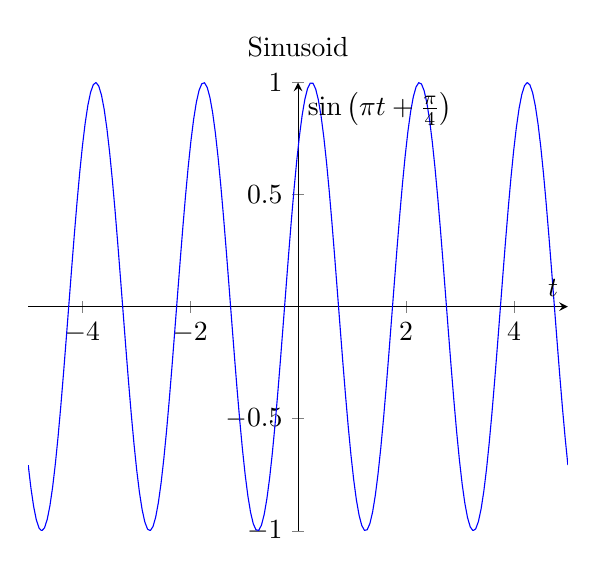
\begin{tikzpicture}
        \begin{axis}[
            xlabel=\(t\), ylabel=\(\sin\left(\pi t + \frac{\pi}{4}\right)\),
            title=Sinusoid,
            axis lines=middle,
            ymin=-1, ymax=1
        ]
        \addplot[
            domain=-5:5,
            samples=200,
            color=blue
        ]{sin(pi*deg(x)+deg(pi/4))};
        \end{axis}
    \end{tikzpicture}
\end{center}

\subsection{}

\begin{center}
    \begin{tikzpicture}
        \begin{axis}[
            xlabel=\(t\), ylabel=\(e^{2t} u(-t)\),
            title=Exponential Unit Step,
            axis lines=middle,
            ymin=0, ymax=1
        ]
        \addplot table[
            mark=none,
            col sep=comma,
            x=t, y=exp
        ]{e5.csv};
        \end{axis}
    \end{tikzpicture}
\end{center}

\subsection{}

\begin{center}
    \begin{tikzpicture}
        \begin{axis}[
            xlabel=\(n\), ylabel=\(e^{-n} u(n)\),
            title=Discrete Exponential Unit Step,
            axis lines=middle,
            ymin=0, ymax=1
        ]
        \addplot[ycomb, mark=*, color=blue] table[
            col sep=comma,
            x=t, y=exp
        ]{e6.csv};
        \end{axis}
    \end{tikzpicture}
\end{center}

\end{document}
